\section{Development}
Development was tracked using a diary See Appendix S.
\newline
We will discuss the Technologies that were used during development and the reasons they were used. We will then take a walk through 
each sprint and discuss the development work done during each.
\subsection{Technologies}
\subsubsection{Front-end}
\paragraph{React.js} \cite{react} Is a front-end application framework, it's benefits include the ability to segment code into 
components that can be reused throughout the application and it's speed in the browser, due to optimisations in it's bundling features. It was chosen 
due to these benefits and the fact the student had previous experience using it. 
There was a possibility of using another framework such as AngularJS \cite{angularjs} but as it is entering end of life in favour of the TypeScript 
version of Angular and the student had little experience with TS it felt more appropriate to use React.js.
\paragraph{Prism.js} \cite{prism} is a javascript highlighting library. It was chosen due to it's various themes and the speed of execution.
\subsubsection{Back-end}
A javascript based backend was chosen to ensure compatibility between the front-end and back-end of the system.
\paragraph{Node.js} \cite{node.js} is a javascript framework, it was chosen for it's massive amount of packages and the students experience in 
using it.
\paragraph{Express.js} \cite{express} is a node backend framework, it was chosen for it's simplicity of hoisting the static files to the 
server.

\subsection{Sprint 1}
The first sprint was interrupted due to the student catching covid. Despite this the student created a baseline for development, creating the basis of the
web application. A React.js\cite{react} front end was created using the React.js tool of Create-react-app \cite{createReactApp}. Simple backend infrastructure was
created, a node.js\cite{node.js} application using express.js\cite{express} to serve the static webpage created from React.js.
\subsection{Sprint 2}
Using a website from my research \cite{astexplorer} as inspiration the student created initial designs as shown in Figures
~\ref{fig:codeeditor1} ~\ref{fig:codeeditor2} ~\ref{fig:codeeditor3} ~\ref{fig:codeeditor4} ~\ref{fig:codeeditor5}
~\ref{fig:codeeditor7}.
These designs were created with the understanding that the code-editor should be as large as possible to allow
the user to edit freely.
\begin{figure}
    
\includegraphics[width=.4\textwidth]{appendix/N/code-editor1.png}
    \caption{Code editor designs See Appendix N}
    \Description{Code editor designs See Appendix N}
    \label{fig:codeeditor1}
\end{figure}
\begin{figure}
    
\includegraphics[width=.4\textwidth]{appendix/N/code-editor2.png}
    \caption{Code editor designs See Appendix N}
    \Description{Code editor designs See Appendix N}
    \label{fig:codeeditor2}
\end{figure}
\begin{figure}
    
\includegraphics[width=.4\textwidth]{appendix/N/code-editor3.png}
    \caption{Code editor designs See Appendix N}
    \Description{Code editor designs See Appendix N}
    \label{fig:codeeditor3}
\end{figure}
\begin{figure}
    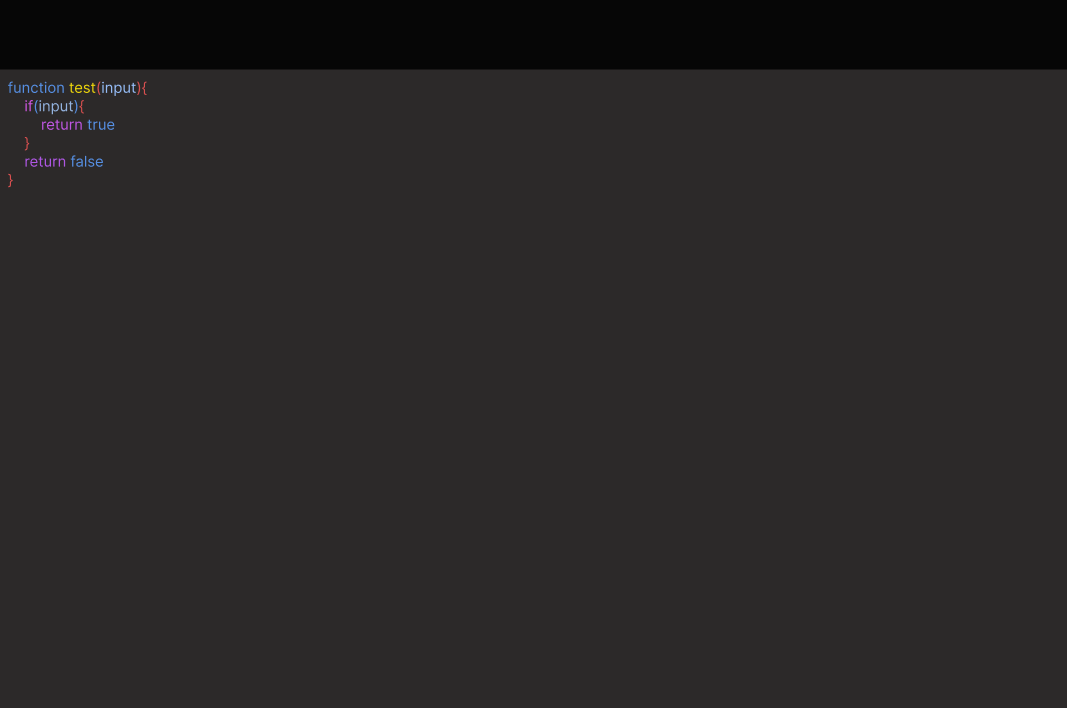
\includegraphics[width=.4\textwidth]{appendix/N/code-editor4.png}
    \caption{Code editor designs See Appendix N}
    \Description{Code editor designs See Appendix N}
    \label{fig:codeeditor4}
\end{figure}
\begin{figure}
    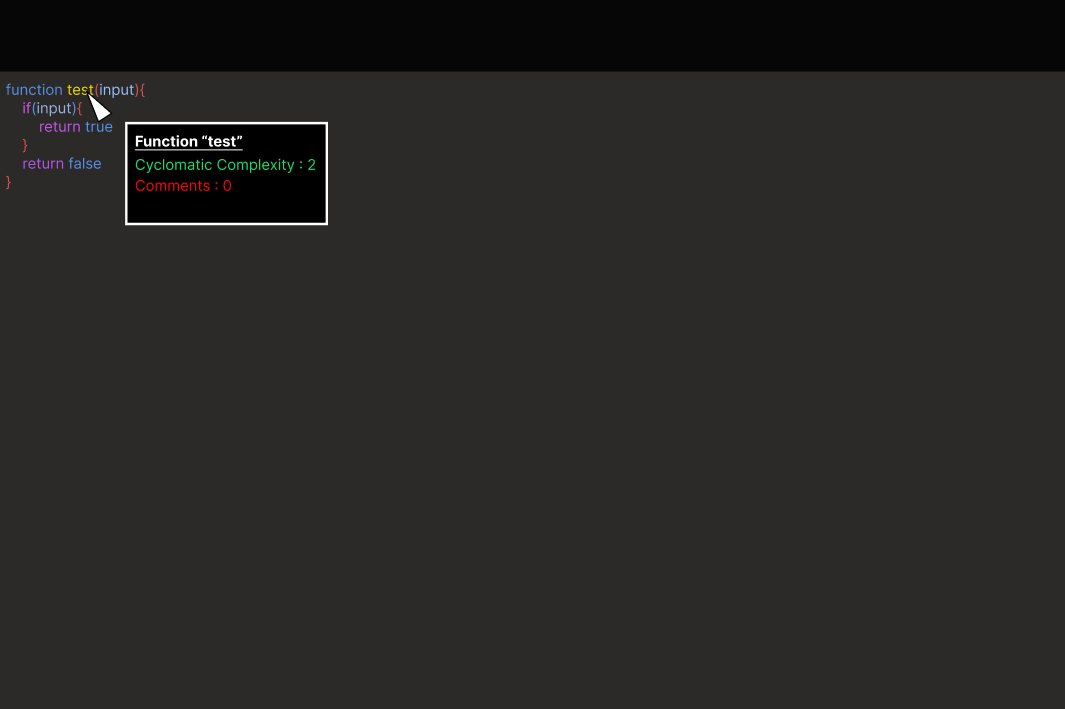
\includegraphics[width=.4\textwidth]{appendix/N/code-editor5.png}
    \caption{Code editor designs See Appendix N}
    \Description{Code editor designs See Appendix N}
    \label{fig:codeeditor5}
\end{figure}
\begin{figure}
    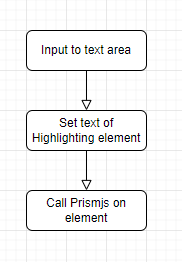
\includegraphics[width=.4\textwidth]{appendix/N/code-editor-activity-diagram.png}
    \caption{Code editor activity diagram See Appendix N}
    \Description{Code editor activity diagram See Appendix N}
    \label{fig:codeeditor6}
\end{figure}
\begin{figure}
    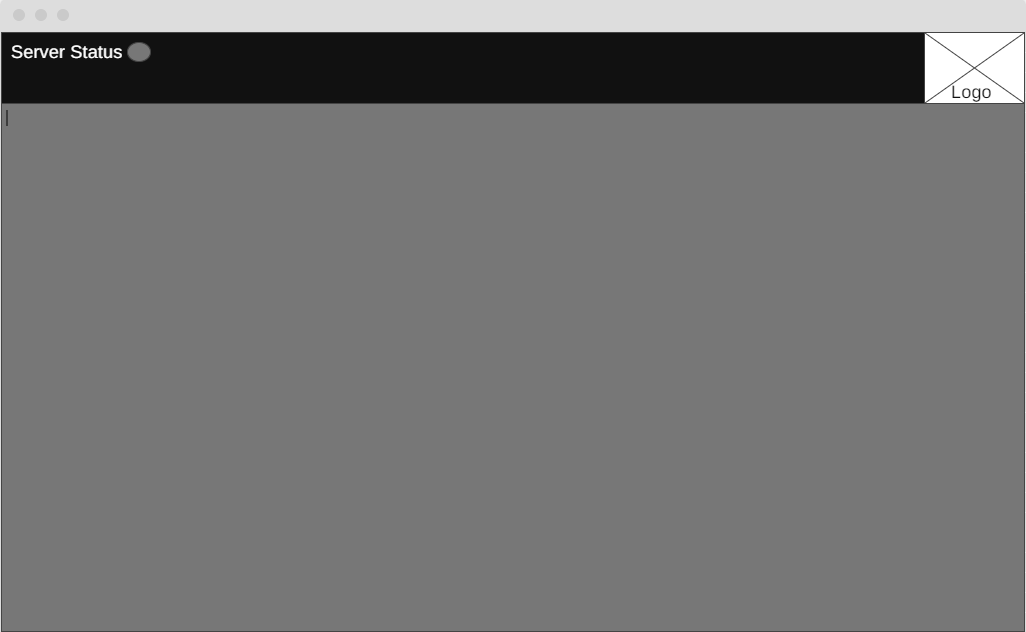
\includegraphics[width=.4\textwidth]{appendix/N/wireframe1.png}
    \caption{Code editor wireframe See Appendix N}
    \Description{Code editor wireframe See Appendix N}
    \label{fig:codeeditor7}
\end{figure}

The next step was to highlight the code entered, with the research into prism.js \cite{prism} it seemed perfect for use
in highlighting the code. The only problem is that prism.js is intended for highlighting static code
These items are also described in the User Stories Appendix as seen on the prism.js Examples page. An excellent article was found written by
Oliver Geer \cite{olivergeer} describing the process of having a textarea above a highlighted code element.

\begin{figure}[h]
    \begin{lstlisting}[language=Javascript]
<textarea
    ref={this.state.editingRef}
    placeholder="Enter Code Here "
    className={styles.editing}
    spellCheck="false"
    onChange={(ev) => {
        this.handleInput(ev);
    }}
    onScroll={(ev) => {
        this.handleScroll(ev);
    }}
    onKeyDown={(ev) => {
        this.handleKeyDown(ev);
    }}
></textarea>
<pre
    ref={this.state.highlightingRef}
    className={styles.highlighting}
    aria-hidden="true"
    >
<code className="language-javascript" id="highlighting-content">
    {this.state.text}
</code>
    \end{lstlisting}
    \caption{React code for code editor from "/client/src/components/code\textunderscore{}editor/CodeEditor.jsx" See Appendix K}
    \Description{React code for code editor from "/client/src/components/code\textunderscore{}editor/CodeEditor.jsx" See Appendix K}
    \label{fig:react-codeeditor}
\end{figure}

As shown in Figure \RefFig{fig:react-codeeditor} the textarea has events attached in the react fashion \cite{reactEvents}. Both elements have
React Refs \cite{reactRefs} attached to allow us to access the elements throughout our React Component.
\begin{figure}[h]
    \begin{lstlisting}[language=Javascript]
handleInput(event) {
    event.persist(); // stops react from recycling the SyntheticEvent on re-render
    let text = this.state.editingRef.current.value;
    if (text[text.length - 1] == "\n") {
        text += " ";
    }
    this.setState({ text });
}
handleKeyDown(event) {
    if (event.key === "Tab") {
      event.preventDefault();
      this.handleTab();

      return;
}

handleTab() {
    let text = this.state.text;

    let before = text.slice(0, this.state.editingRef.current.selectionStart);
    let after = text.slice(
      this.state.editingRef.current.selectionEnd,
      text.length
    );
   
    let cursor = this.state.editingRef.current.selectionStart + 1;
    console.log(cursor);
    
    let newText = before + "\t" + after;
    

    this.state.editingRef.current.value = newText;
    this.setState({ text: newText }, () =>this.state.editingRef.current.setSelectionRange(cursor, cursor));
  }
    \end{lstlisting}
    \caption{Event handlers for code editor from "/client/src/components/code\textunderscore{}editor/CodeEditor.jsx" See Appendix K}
    \Description{Event handlers for code editor from "/client/src/components/code\textunderscore{}editor/CodeEditor.jsx" See Appendix K}
    \label{fig:event-handlers}
\end{figure}
When the onChange listener is fired on the textarea, the text from the text is set to state so we can access in our render function. 
We add an extra character to the text as a code block will ignore an empty line as shown in Figure \RefFig{fig:event-handlers}.
\newline
On a key event being fired we check if tab is the key pressed, if it is we cancel the tabbing by calling "event.preventDefault()" \cite{preventDefault}.
We then get the cursor position and insert a tab between before and after the selection. as shown in Figure \RefFig{fig:event-handlers}.

We set the state to the new text, starting the previous process again and then in the callback of setState \cite{reactSetState} 
we update the cursor position.
\newline

This is all tied together by the process described by Figure \RefFig{fig:codeeditor6}. The code set to state is used in the render function and applied 
to the code element as shown in Figure \RefFig{fig:final-steps} by specifying "this.state.text". After the render function completes 
a special react function activates "componentDidUpdate" \cite{reactDidUpdate} which is called by react when the component updates e.g. via a state update. So once we set the text we can call 
highlight on it.

\begin{figure}[h]
    \begin{lstlisting}[language=Javascript]
<code className="language-javascript" id="highlighting-content">
    {this.state.text}
</code>

componentDidUpdate() {
    setTimeout(() => Prism.highlightAll(), 0);
  }

    \end{lstlisting}
    \caption{Final steps of creating highlighted text from  "/client/src/components/code\textunderscore{}editor/CodeEditor.jsx" See Appendix K}
    \Description{Final steps of creating highlighted text from "/client/src/components/code\textunderscore{}editor/CodeEditor.jsx" See Appendix K}
    \label{fig:final-steps}
\end{figure}

\subsection{Sprint 3}
The focus for Sprint 3 was to get the deployment sorted for user testing, there was a problem here. The css for highlighting using prism was not working 
when using a development build. The problem was that the bundler was packaging the scss files as modules, meaning that prism styling wasn't being applied. 
Scss modules are beneficial when using multiple components as you can specify the same class name and have them bundled differently. The fix for this was to 
update the react version as this was a bug fixed in a newer version. An overlay was added to inform the user of the testing procedure.
The code-editor was then deployed to heroku 
\href{https://cq-code-editor-testing.herokuapp.com/}{https://cq-code-editor-testing.herokuapp.com/} and a questionnaire was sent out to potential users.

\subsubsection{Parser Course.}
During this sprint the student realised they were lacking knowledge on the implementation of a parser so the student enrolled themselves in a course 
Building a parser from scratch by Dmitry Soshnikov \cite{parserCourse} which is aimed at teaching the basics of compilers by creating 
a parser for a hypothetical language. The rest of the sprint was used following this course.


\subsection{Sprint 4}
The student completed the course on parsing and started on creating their own version of the parser. As previously described in the background section. This 
would be a \textbf{Top-down Recursive Descent Parser}. Taking the knowledge from the course and expanding on it to create a JavaScript parser.
\begin{figure}[h]
    \begin{lstlisting}[language=Javascript]
/**
* Initial Parse Function
* 
* 
* Starts tokenizer and updates lookahead
* 
* 
* Starts parsing from Program
* 
* Attaches comments if available
* @param {string} input - Input string of source code
* @returns {object} - Program AST 
*/
parse(input) {
    this.source = input;
    this.tokenizer.update(this.source)
    this.lookahead = this.tokenizer.next();
    const ast = this.Program()
    if (this.tokenizer.comments.length) {
        ast.comments = this.tokenizer.comments
    }
    return ast
}
   
/**
* Program:
* 
*      -> StatementList
* @returns {object} Program AST
*/
Program() {
    return {
        type: AST_TYPES.Program,
        body: this.StatementList()
    }
}   
    \end{lstlisting}
    \caption{Initial parser steps  See Appendix O}
    \Description{Initial parser steps  See Appendix O}
    \label{fig:parser1}
\end{figure}
\subsubsection{Tokenising.}
Tokenising is the initial stage of parsing, we need to create tokens for our parser to parse. 
The student utilised a Regular Expression \cite{regexp} array to create a token hierarchy as seen in Figure \RefFig{fig:tokenHierarchy} where regular expressions are 
matched with their corresponding token See TOKEN\textunderscore{}CONST\textunderscore{}TYPES.js in Appendix Q. This is then looped through by the tokeniser and if the token is not 
not found within the hierarchy an error is raised, if it is found it is checked for special cases e.g. the multi line string where the location must 
be handled because of the column and line tracking. Then the token is returned. See Figure \RefFig{fig:tokeniser}.
\begin{figure}[h]
    \begin{lstlisting}[language=Javascript]
        if (type === TOKEN_TYPES.MULTI_LINE_STRING) {
            this.handleMultiLine(tokenValue)
            type = TOKEN_TYPES.STRING; // we've handled the multilines so just treat as a string
        }
        return {
            type: type,
            value: tokenValue,
            loc: { start: pos, end: this.position() },
        }
    }
throw new ParseSyntaxError(`Unexpected token: "${cur[0]}" at ${pos.line}:${pos.column}`, 
        { type: "Unknown", value: cur[0], loc: { start: pos, end: pos } })
    \end{lstlisting}
    \caption{Tokeniser.js  See Appendix Q}
    \Description{Tokeniser.js  See Appendix O}
    \label{fig:tokeniser}
\end{figure}
\begin{figure}[h]
    \begin{lstlisting}[language=Javascript]
const TOKEN_SPEC = [
    [/^\n/, TOKEN_TYPES.NEWLINE], // caught by below, must come before
    [/^\s/, TOKEN_TYPES.WHITESPACE],
    [/^\/\/.*/, TOKEN_TYPES.SINGLE_LINE_COMMENT],
    [/^\/\*[\s\S]*?\*\//, TOKEN_TYPES.MULTI_LINE_COMMENT],
    \end{lstlisting}
    \caption{tokenHierarchy.js  See Appendix Q}
    \Description{tokenHierarchy.js  See Appendix O}
    \label{fig:tokenHierarchy}
\end{figure}
\subsubsection{Parsing.}
In Figure \RefFig{fig:parser1} we see the parse function that starts everything, our grammar starts from the Program node which has the grammar 

\begin{verbatim}
    Program
        StatementList
\end{verbatim}
This again shows the similarity between our final code and the Grammar as described in the background section. In Figure \RefFig{fig:parser2} we parse a 
StatementList which is added to based on the null check performed in Figure \RefFig{fig:parser3} because we eat semicolons and newlines as if they were empty statements 
and don't add them to the parse tree, otherwise a normal statement is added from the grammar definition. We keep following the grammar tree down until we get to 
the most basic of elements which is the Literal as shown in \RefFig{fig:parser4}.
\newline
In each of these examples we can see a few things, the use of the lookahead to determine the type, this is the predictive element of the parser and the use of 
AST\textunderscore{}TYPES which is a constant file used to aid development which specifies the string names of all the AST node types See Appendix P.
\begin{figure}[h]
    \begin{lstlisting}[language=Javascript]
        /**
        * StatementList
        * 
        *      StatementList Statement -> Statement ...
        * @param {string}[d=null] stopLookingPast 
        * @returns {Object[]} Array of Statements
        */
       StatementList(stopLookingPast = null) {
           let list = this.addStatementIfNotNull([])
           while (this.lookahead.type !== TOKEN_TYPES.EOF && this.lookahead.type !== stopLookingPast) {
               list = this.addStatementIfNotNull(list)
           }
           return list
       }
   
       /**
        * Attempt to parse statement and add to list if not null
        * @param {Array} list StatementList
        * @returns {Array} StatementList
        */
       addStatementIfNotNull(list) {
           const statement = this.Statement()
           if (statement != null) {
               list.push(statement)
           }
           return list
       }
    \end{lstlisting}
    \caption{StatementList parsing See Appendix O}
    \Description{StatementList parsing  See Appendix O}
    \label{fig:parser2}
\end{figure}
\begin{figure}[h]
    \begin{lstlisting}[language=Javascript]
        /**
        * Statement 
        * 
        *      : ExpressionStatement
        *      | ForStatement
        *      | DoWhileStatement
        *      | WhileStatement
        *      | ReturnStatement
        *      | ClassDeclaration
        *      | FunctionDeclaration
        *      | VariableStatement
        *      | BlockStatement
        *      | IfStatement       
        *      | null : EOF | SEMI_COLON | NEWLINE
        *      
        * @returns {Object} Statement
        */
       Statement() {
           if (this.lookahead.type === TOKEN_TYPES.EOF) {
               return null
           }
           switch (this.lookahead.type) {
               case TOKEN_TYPES.SEMI_COLON:
                   this.eat(TOKEN_TYPES.SEMI_COLON);
                   return null;
               case TOKEN_TYPES.NEWLINE:
                   this.eat(TOKEN_TYPES.NEWLINE);
                   return null
    \end{lstlisting}
    \caption{Statement parsing See Appendix O}
    \Description{Statement parsing  See Appendix O}
    \label{fig:parser3}
\end{figure}
\begin{figure}[h]
    \begin{lstlisting}[language=Javascript]
        /**
        * Literal propretor 
        * 
        * Literal
        * 
        *      :NumericLiteral
        *      :StringLiteral
        *      :BooleanLiteral
        *      :NullLiteral
        * 
        * @throws {ParseSyntaxError} Throws error on unexpected literal production
        * @returns {Object} Literal 
        */
       Literal() {
           switch (this.lookahead.type) {
               case TOKEN_TYPES.NUMBER:
                   return this.NumericLiteral();
               case TOKEN_TYPES.STRING:
                   return this.StringLiteral();
               case TOKEN_TYPES.TRUE:
                   return this.BooleanLiteral(this.lookahead.type);
               case TOKEN_TYPES.FALSE:
                   return this.BooleanLiteral(this.lookahead.type);
               case TOKEN_TYPES.NULL:
                   return this.NullLiteral();
           }
           /* istanbul ignore next */
           const loc = this.lookahead == null ? "" : `at ${this.lookahead.loc.start.line}:${this.lookahead.loc.start.col}`;
           /* istanbul ignore next */
           const type = this.lookahead == null ? "unknown" : `"${this.lookahead.type}"`;
           /* istanbul ignore next */
           throw new ParseSyntaxError(`Unexpected literal production of type: ${this.lookahead.type} : ${this.lookahead.value} at ${this.lookahead.loc.start.line}:${this.lookahead.loc.start.column}`, this.lookahead)
       }       
    \end{lstlisting}
    \caption{Literal parsing See Appendix O}
    \Description{Literal parsing  See Appendix O}
    \label{fig:parser4}
\end{figure}
\newline
\subsubsection{Testing.} Testing was performed using jest \cite{jest} and used to test every part of the parser. All of the testing suites used a test table which 
which allowed multiple tests to be run in the same suite with similar descriptions. In \RefFig{fig:test} the test checks that the program parses 
an empty statement correctly. "testTable" is an array of arrays which contain ["input",{expected}].
\begin{figure}[h]    
\begin{lstlisting}[language=Javascript]
        import Parser from "../Parser"
        // table of tests [program,expectedOutput]
        const testTable = [
            [
                `;
        `, {
                    "type": "Program",
                    "body": []
                }
            ]
        
        ]
        
        
        
        
        const parser = new Parser()
        describe('Testing empty statement', () => {
            describe.each(testTable)('parsing %s', ((program, expected) => {
        
                test(`returns ${JSON.stringify(expected)}`, () => {
                    expect(parser.parse(program)).toEqual(expected)
                })
            }))
        
        })
    \end{lstlisting}
    \caption{Example test  See Appendix R}
    \Description{Example test  See Appendix R}
    \label{fig:test}
\end{figure}
\subsection{Sprint 5}
Sprint 5 continued with progress on the parser. More javascript support was added, including the ability for statements to be ended by 
newlines, unary and not operators, functions declarations, iteration statements, javascript class definitions, function calls and finally memmber expressions.

There was also AutoComplete and autofill functionality added due to user testing, this will be described in user evaluation.

Finally the rest of focus was used on the creation of the evaluation metrics, this was made quite simple by the use of the created AST.
Cyclomatic Complexity was analysed by using the visitor pattern to crawl through the AST node and increment the complexity when finding a jumping statement, see appendix T /complexity/cyclomatic.js.
Halstead Complexity was analysed by crawling through the entire AST and finding the operands and operators, see Appendix T /complexity/halstead.js. Both of these are tested in Appendix T /complexity/complexity.test.js
\newline
These are both called by evaluate.js which also checks class complexity measures, SLOC errors and function param errors. The tests for this can be found in Appentix T "evaluate.test.js"
\newpage

